\section{Thuật toán Alpha Skip Search}

\subsection{Đặc điểm chính}
Alpha Skip Search là một cải tiến của thuật toán Skip Search. Thay vì xây dựng bucket cho từng ký tự đơn lẻ trong mẫu, thuật toán xây dựng bucket cho các nhân tố có độ dài $log_{\sigma}(m)$ xuất hiện trong mẫu. Nhờ xét một đoạn ký tự thay vì một ký tự, thuật toán có thể giảm số vị trí ứng viên cần kiểm tra trong giai đoạn tìm kiếm.

Ý tưởng chính của Alpha Skip Search là sử dụng trie để lưu trữ các nhân tố có cùng độ dài trong mẫu, sau đó liên kết mỗi nhân tố với danh sách các vị trí mà nhân tố đó xuất hiện. Cách tiếp cận này giúp cải thiện hiệu quả trung bình của Skip Search, đặc biệt khi mẫu đủ dài và bảng chữ cái có kích thước cố định.

Thuật toán có các đặc điểm sau:

\begin{itemize}
    \item là một cải tiến của thuật toán Skip Search;
    \item sử dụng bucket lưu vị trí xuất hiện của từng nhân tố độ dài $log_{\sigma}(m)$ trong mẫu;
    \item giai đoạn tiền xử lý có độ phức tạp thời gian và không gian $O(m)$;
    \item giai đoạn tìm kiếm có độ phức tạp thời gian $O(nm)$;
    \item số phép so sánh ký tự văn bản kỳ vọng là:
    \[
    O(log_{\sigma}(m) \frac{n}{m - log_{\sigma}(m)})
    \]
\end{itemize}

\subsection{Mô tả thuật toán}

Giai đoạn tiền xử lý của thuật toán Alpha Skip Search bao gồm việc xây dựng một trie $T(x)$ chứa tất cả các nhân tố có độ dài:

\[
\ell = log_{\sigma}(m)
\]

xuất hiện trong mẫu $x$. Các lá của trie $T(x)$ biểu diễn toàn bộ các nhân tố độ dài $\ell$ của $x$. Với mỗi lá của trie, thuật toán tạo ra một bucket tương ứng để lưu danh sách các vị trí mà nhân tố gắn với lá đó xuất hiện trong $x$.

Nếu kích thước bảng chữ cái được xem là hằng số, thời gian tiền xử lý trong trường hợp xấu nhất là tuyến tính.

Giai đoạn tìm kiếm bao gồm việc tra cứu các bucket tương ứng với các nhân tố văn bản:

\[
y[j \ldots j + \ell - 1]
\]

với mọi vị trí:

\[
j = k(m - \ell + 1) - 1,
\]

trong đó $k$ là số nguyên thuộc khoảng:

\[
1 \leq k \leq \left\lfloor \frac{n-\ell}{m} \right\rfloor.
\]

Giai đoạn tìm kiếm có độ phức tạp thời gian bậc hai trong trường hợp xấu nhất, nhưng số phép so sánh ký tự văn bản kỳ vọng là:

\[
O(log_{\sigma}(m) \frac{n}{m - log_{\sigma}(m)}).
\]

\subsection{Cài đặt bằng C++}
\begin{verbatim}
#include <iostream>
#include <vector>
#include <string>
#include <array>

using namespace std;

const int ASIZE = 256;

/* ---------- Trie Node ---------- */
struct TrieNode {
    array<int, ASIZE> next;
    vector<int> bucket;

    TrieNode() {
        next.fill(-1);
    }
};

/* ---------- Alpha Skip Search with Trie ---------- */
void AlphaSkipSearchTrie(const string &pat, const string &txt, int alphabetSize) {
    int m = pat.length();
    int n = txt.length();

    if (m == 0 || n < m) {
        return;
    }

    /* Compute log_sigma(m) */
    int logM = 0;
    int temp = m;

    while (temp > alphabetSize) {
        ++logM;
        temp /= alphabetSize;
    }

    if (logM == 0) {
        logM = 1;
    }

    vector<TrieNode> trie;
    trie.emplace_back(); // root = 0

    /* ---------- Preprocessing ---------- */
    for (int i = 0; i <= m - logM; ++i) {
        int node = 0;

        for (int k = 0; k < logM; ++k) {
            unsigned char c = (unsigned char)pat[i + k];

            if (trie[node].next[c] == -1) {
                trie[node].next[c] = trie.size();
                trie.emplace_back();
            }

            node = trie[node].next[c];
        }

        trie[node].bucket.push_back(i);
    }

    /* ---------- Searching ---------- */
    int shift = m - logM + 1;

    for (int j = m + 1 - logM; j <= n - logM; j += shift) {
        int node = 0;

        for (int k = 0; k < logM; ++k) {
            unsigned char c = (unsigned char)txt[j + k];

            node = trie[node].next[c];

            if (node == -1) {
                break;
            }
        }

        if (node == -1) {
            continue;
        }

        for (int pos : trie[node].bucket) {
            int start = j - pos;

            if (start < 0 || start > n - m) {
                continue;
            }

            bool match = true;

            for (int k = 0; k < m; ++k) {
                if (pat[k] != txt[start + k]) {
                    match = false;
                    break;
                }
            }

            if (match) {
                cout << "Pattern found at index: "
                     << start << endl;
            }
        }
    }
}

/* ---------- Main ---------- */
int main() {
    string text = "ACGTACGTGACGTACGT";
    string pattern = "ACGT";

    int alphabetSize = 4; // Ví dụ DNA: A, C, G, T

    AlphaSkipSearchTrie(pattern, text, alphabetSize);

    return 0;
}
\end{verbatim}

\subsection{Kiểm nghiệm thuật toán}

\textbf{Pha tiền xử lý:}

\begin{figure}[H]
    \centering
    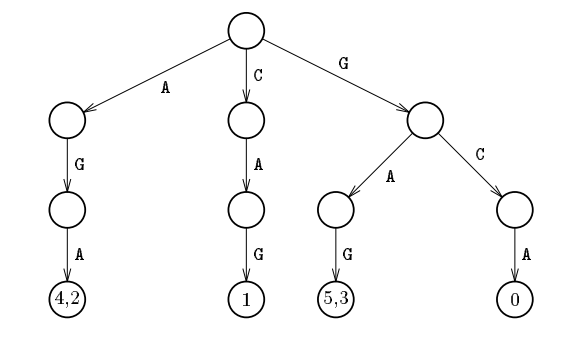
\includegraphics[width=10cm]{Images/2026-05-18-14-53-44.png}
    \caption{Kết quả tiền xử lý của thuật toán Alpha Skip Search}
    \label{fig:alpha-skip-search-preprocess-1}
\end{figure}

\begin{figure}[H]
    \centering
    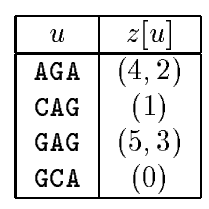
\includegraphics[width=6cm]{Images/2026-05-18-14-53-57.png}
    \caption{Bảng Z sử dụng trong thuật toán Alpha Skip Search}
    \label{fig:alpha-skip-search-preprocess-2}
\end{figure}

Bảng $Z$ được sử dụng bởi thuật toán Alpha Skip Search.

\textbf{Pha tìm kiếm:}

Lần 1:

\begin{figure}[H]
    \centering
    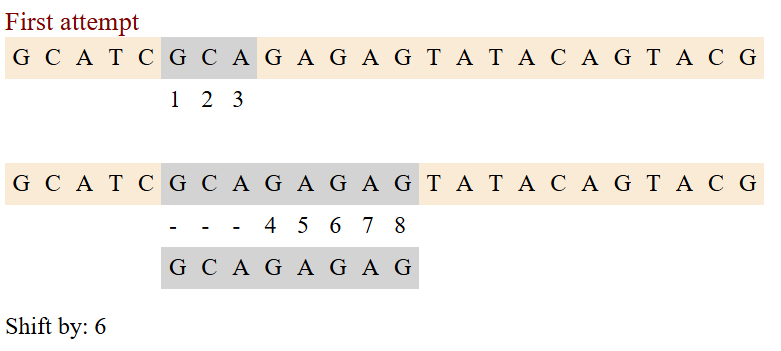
\includegraphics[width=15cm]{Images/2026-05-18-14-54-52.png}
    \caption{Bước 1 trong quá trình thực hiện thuật toán Alpha Skip Search}
    \label{fig:alpha-skip-search-step-1}
\end{figure}

Lần 2:

\begin{figure}[H]
    \centering
    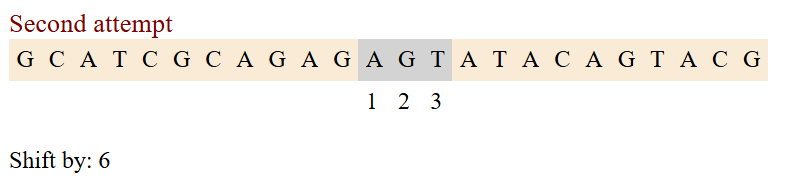
\includegraphics[width=15cm]{Images/2026-05-18-14-55-03.png}
    \caption{Bước 2 trong quá trình thực hiện thuật toán Alpha Skip Search}
    \label{fig:alpha-skip-search-step-2}
\end{figure}

Lần 3:

\begin{figure}[H]
    \centering
    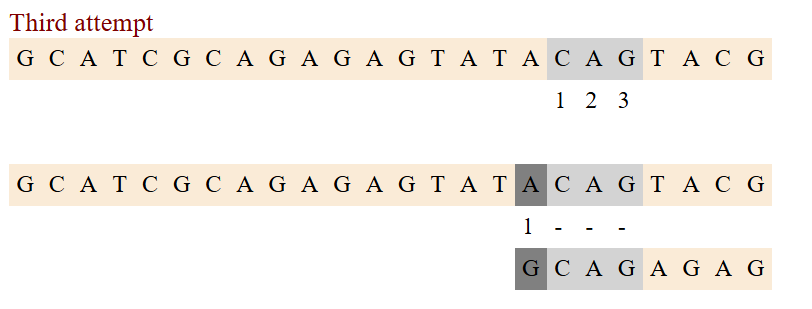
\includegraphics[width=15cm]{Images/2026-05-18-14-55-16.png}
    \caption{Bước 3 trong quá trình thực hiện thuật toán Alpha Skip Search}
    \label{fig:alpha-skip-search-step-3}
\end{figure}

Thuật toán Alpha Skip Search thực hiện 18 lần so khớp chuỗi trong ví dụ trên.